\documentclass[11pt]{article}

\usepackage[utf8]{inputenc}
\usepackage[english]{babel}

\usepackage{hyperref}		  % For \autoref
\usepackage{parskip}		  % Don't indent paragraphs; skip instead.

\usepackage{amsfonts, amsmath, amssymb}
\usepackage{amsthm}
\usepackage{changepage} 	% For adjustwidth environment
\usepackage{colortbl}  		% Provides the  \arrayrulecolor command.
\usepackage{environ}
\usepackage{framed}			  % For leftbar environment
\usepackage{mathtools}		% For the \mathclap command.
\usepackage{ragged2e}		  % FlushLeft environment
\usepackage{thmtools}		  % For restatable environment
\usepackage{varwidth}
\usepackage{xcolor}
\usepackage{makeidx}
\usepackage{bm}           % For vector bold
\usepackage[margin=3cm]{geometry}


\newenvironment{indentone}{\begin{adjustwidth}{3em}{0em}}{\end{adjustwidth}}

% \renewcommand{\bfseries}{\scshape}
% \usepackage{ccfonts}
\newcommand\op[1]{{\ \mathrm{#1}\ }}
\newcommand\uop[1]{{\mathrm{#1}}}

\newcommand\AND{{\op{AND}}}
\newcommand\IMPLIES{{\op{IMPLIES}}}
\newcommand\MYS{{\op{MYS}}}
\newcommand\OR{{\op{OR}}}
\newcommand\NOT{{\uop{NOT}}}
\newcommand\XOR{{\op{XOR}}}
\newcommand\IFF{{\op{IFF}}}
\newcommand\VEC{\bm}{}
\newcommand\DIV{\>|\>}

\newcommand\FALSE{{\mathrm{F}}}
\newcommand\TRUE{{\mathrm{T}}}

% Number sets
\newcommand{\Nats}{\mathbb N}		% Naturals
\newcommand{\Ints}{\mathbb Z}		% Integers
\newcommand{\Q}{\mathbb Q}			% Rationals
\newcommand{\R}{\mathbb R}			% Reals
\newcommand{\C}{\mathbb C}			% Complexes
\newcommand{\cO}{\mathcal O}		% Big-Oh
\newcommand{\cP}{\mathcal P}		% Power set

\theoremstyle{definition}
\newtheorem{theorem}{Theorem}[section]
\newtheorem{corollary}{Corollary}[section]
\newtheorem{lemma}{Lemma}[section]
\newtheorem{proposition}{Proposition}[section]
\newtheorem{definition}{Definition}[section]
\newtheorem{remark}{Remark}[section]
\newtheorem{example}{Example}[section]
\newtheorem{question}{Question}[section]
\newtheorem{problem}{Problem}[section]
\newtheorem{exercise}{Exercise}[section]
\newtheorem{homework}{Homework}[section]
\newtheorem{algorithm}{algorithm}[section]
\numberwithin{equation}{section}
% \newtheorem*{corollary}{Corollary}
% \newtheorem*{theorem}{Theorem}
% \newtheorem*{definition}{Definition}
% \newtheorem*{remark}{Remark}


% Essential sections of notes, e.g. definitions/theorems.
\NewEnviron{bigbox}{{

    \newdimen\slidewidth
    \slidewidth=\linewidth
    % Without this, I get errors beginning "Overfull \hbox (6.79999pt too
    % wide)"
    \advance\slidewidth by -7pt

    \medskip

    \fbox{parbox{\slidewidth}{\BODY}}

    \medskip

  }}

% Stuff I should write or draw during lecture. (from James)
% Additional notes


\NewEnviron{writenotes}{\vspace{1ex}\begin{leftbar}{\BODY}\end{leftbar}}

\title{Notes\\
  {\large STA302H1 - Fall 2020}}
\author{Ziyue Yang}

\begin{document}
\maketitle

\tableofcontents

\newpage

\section{Module 9 - Multiple Linear Regression Analysis}
\subsection{Review}
\textbf{Multiple Linear Regression}
\begin{itemize}
\item MLR Model (to obtain using the least-squares estimation):
\begin{equation}
  \VEC{Y} = \VEC{X\beta} + \VEC{e},
\end{equation}
where
\begin{indentone}
$\VEC{Y}\in M_{n\times 1}$, 

$\VEC{X}\in M_{n\times(p+1)}$,

$\VEC{\beta}\in M_{p+1}$,

$\VEC{e}\in M_{n\times 1}$,

\end{indentone}

\item $p$ predictors: $p+1$ $\VEC{\beta}$'s
\item Gauss-Markov Conditions: $E(\VEC{e})=0, Var(\VEC{e})=\sigma^2 I$
\item Normal Error assumption (for inference)
\end{itemize}

\subsection{$R^2$ and Adjusted $R^2$}

\begin{definition}[$R^2$: Coefficient of Multiple Determination]
  \begin{equation}
  R^2=\frac{SSReg}{SST}=1-\frac{RSS}{SST} = \frac{\VEC{Y'(H-\frac{1}{n} J)Y}}{\VEC{Y'(I-\frac{1}{n}J)Y}}
  \end{equation}

  called the coefficient of multiple determination (in the MLR setting).

  $R^2$ gives the percentage of variation in $Y$ explained by the model with all the $p$ predictors.
\end{definition}
\begin{writenotes}
  Note that it's NOT the square of a sample correlation coefficient ($r^2$) anymore.
\end{writenotes}

\begin{remark}
For the same $Y$, as $p$ increases, 

\begin{indentone}
  SST remains the same,

  SSReg stays the same or increases,

  RSS stays the same or decreases, 
\end{indentone}

hence $R^2$ either stays the same or increases.
\end{remark}

\begin{question}
  Is $R^2$ helpful in telling whether additional predictors are \textit{useful} for explaining the response?

  No.
\end{question}

\begin{definition}[Adjusted $R^2$]
  \begin{equation}
    R^2_{adj} = 1- \frac{RSS/(n-p-1)}{SST/(n-1)} = 1 - (n-1)\frac{MSE}{SST}
  \end{equation}

  where $S^2=\frac{RSS}{n-p-1}$ is an unbiased estimate of $\sigma^2=Var(e_i)=Var(Y_i)$.
  \begin{itemize}
    \item adjusted for the number of predictors in the model
    \item better to use instead of $R^2$
    \item always: $R^2_{adj} < R^2$ (note that the inequality is strict) 
  \end{itemize}
\end{definition}
\begin{writenotes}
  Case. $p > 1$ (MLR)
  \begin{indentone}
    Then $(n-1)/(n-p-1) > 1$
  \end{indentone}
  General case: as $p$ increases (adding more predictors to the model), $(n-1)/(n-p-1)$ increases.
\end{writenotes}

\subsection{Global and Partial F-tests}
\subsubsection{Motivational Examples: Salary vs. Experience, Wine Quality}
\begin{definition}[Global F-test]
  Testing Hypotheses: for $j=1\dots p$,
  \begin{gather}
    H_0: \beta_1=\beta_2=\dots=\beta_p=0\\
    H_a: \text{at least one } \beta_j \text{ is not } 0
  \end{gather}
  To test whether there is a linear association between $Y$ and all predictors.

  Test statistic:
  \begin{equation}
    F_{obs} = \frac{MSReg}{MSE}=\frac{SSReg/p}{RSS/(n-p-1)}
  \end{equation}

  Under $H_0$, $F_{obs}$ is an observation from the $F$ distribution with $df=(p,n-p-1)$.

  Hence we can conclude that
  \begin{indentone}
    Small p-value: Rhe model contains at least one significant predictor among the set of $p$ predictors

    Large p-value: None of the $p$ predictors are relevant for estimating/predicting $Y$.
  \end{indentone}
\end{definition}




\newpage

\section{Module 10 - Diagnostics in MLR}

\subsection{Inference for a Single Regression Coefficient}

\subsubsection{Hypothesis Testing}

As in SLR, we are interested in testing

\begin{equation}
  H_0: \beta_j = 0\text{ vs. }H_a: \beta_j\neq 0.
\end{equation}

Test statistic:

\begin{equation}
  t_{obs} = \frac{b_j}{SE(b_j)}
\end{equation}

Under $H_0$, $t_{obs}$ is an observation from the T distribution with $\text{df}=n-p-1$. This test gives an indication of whether or not the $j$th predictor, $X_j,j=1\dots p$, contributes to the prediction of the response variable \textbf{over and above} all the other predictors.

This is the special case of the Partial F-test with $k=1$

\subsubsection{Confidence Interval}

Confidence interval for $\beta_j, j=1\dots p$, assuming all the other predictors are in the model, is

\begin{equation}
  \beta_j \pm t_{\alpha/2, n-p-1}SE(b_j),
\end{equation}
(i.e. unbiased estimate $\pm$ Margin of Error, where MOE is the critical value $\times$ std error).

where
\begin{itemize}
  \item $b_j$: unbiased estimator of $\beta_j$
  \item $SE(b_j)$: standard error of the estimator
  \item $t_{\alpha/2, n-p-1}$: critical value of $100(1-\alpha/2)$th quantile from the T distribution with $\text{df}=n-p-1$.
\end{itemize}

\subsubsection{Global F-test vs. Individual t-tests}
\begin{itemize}
\item In SLR, these tests are equivalent
\item In MLR, the global F-test is designed to test the \textit{overall model}, while the $t$-tests are designed to test \textit{individual coefficients}.
\end{itemize}

\textbf{Case A.} If the Global F-test is significant and:
\begin{itemize}
\item A.1: All or some or the t-tests are significant, $\implies$ there are some useful explanatory variables for predicting $Y$.
\item A.2: All the t-tests are not significant, $\implies$ this is an indication of "multicollinearity", i.e. strongly correlated $X$'s.

This implies that individual X's do not contribute to the prediction of Y over and above other $X$'s.
\end{itemize}

\textbf{Case B.} If the Global F-test is NOT significant and:
\begin{itemize}
\item B.1: All the t-tests are not significant, $\implies$ none of the $X$'s contributes to the prediction of $Y$.
\item B.2: Some of the $t$-tests are significant, $\implies$
\begin{itemize}
\item The model has no predictive ability. Likely, if there are many predictors, there are type I errors in the $t$-tests.
\item The predictors are poorly chosen. The contribution of one useful predictor among many poor ones may not be enough for the model (Global F-test) to be significant.
\end{itemize}
\end{itemize}


\subsection{Multicollinearity}

\begin{definition}
  Multicollinearity occurs when explanatory variables are highly correlated.
\end{definition}
\begin{writenotes}
  In this case, it is difficult to measure the individual influence of one of the predictors on the response.
\begin{itemize}
\item The fitted equation is unstable
\item The estimated regression coefficients vary widely from data set to data set (even if the data sets are similar) and depending on which predictor is included in the model.
\item The estimated regression coefficients may even have opposite sign than what is expected (\textit{e.g. Simpson's Paradox}).
\end{itemize}
\end{writenotes}

\begin{remark}
  When some $X$'s are perfectly correlated, we cannot estimate $\beta$ because $X'X$ is sigular. Even if $X'X$ is close to singular, its determinant will be close to zero and the standard errors of estimated coefficients will be large.
\end{remark}

\begin{remark}
  For the general multiple regression model
  \begin{gather}
    Y=\beta_0+\beta_1x_1+\beta_2x_2+\dots+\beta_px_p+e\\
    Var(\hat{\beta_j}) = \frac{1}{1-R^2_j}\times\frac{\sigma^2}{(n-1)S^2_{x_j}}, j=1\dots p
  \end{gather}
  where $R_j^2$ is the value of $R^2$ from the regression of $x_j$ on the other $x$'s.
\end{remark}
\begin{writenotes}
  The $j$th Variance Inflation Factor (VIF) $=\frac{1}{1-R^2_j}$

  A commonly used cut-off is 5.
\end{writenotes}

\newpage

\subsection{Diagnostics and Remedies}
\subsubsection{Leverage and Influential Points}
\begin{definition}[Identifying Leverage Points]
Classify the $i$th point as a point of high leverage (i.e. a lvg point) in MLR model with $p$ predictors if
 \begin{equation}
   h_{ii} > 2\times\text{average}(h_{ii}) = 2\times \frac{p+1}{n}
 \end{equation}
\end{definition}
\begin{writenotes}
  In SLR, $p=1, h_{ii} > 2\left(\frac{2}{n}\right)=\frac{4}{n}$.
\end{writenotes}

\begin{remark}
  When a \textbf{valid} model has been fit, a plot of standardized residuals against any predictor or any linear combination of the predictors (e.g. the fitted values) will have the following features:
\begin{enumerate}
  \item A random scatter of points around the horizontal axis, since the mean function of $e_i$ is zero when a \textit{correct model has been fit} (linearity)
  \item Constant variability as we look along the horizontal axis, i.e.
  \begin{equation}
    Var(e)=\sigma^2 I=\begin{pmatrix}\sigma^2&0&\dots&0\\
    0 &\sigma^2&\dots&0\\
    \vdots&\vdots&\ddots&\vdots\\
    0&0&\dots&\sigma^2
    \end{pmatrix}
  \end{equation}

\end{enumerate}
Hence, \textbf{any pattern} in plot of standardized residuals is indicative that an \textbf{invalid} model has been fit to the data. Any nonrandom pattern itself does not provide direct information on how the model is misspecified.
\end{remark}

\subsubsection{The Box-Cox Transformation}

\begin{definition}
The Box-Cox transformation is a general method for transforming a strictly positive (response or predictor) variable.
\end{definition}
\begin{writenotes}
 It aims to find transformation that makes the transformed variable close to normally distributed.

 It considers a family of \textit{power transformations}.

\begin{indentone}Suppose the power to be $\lambda$:
 \begin{itemize}

   \item $\lambda=0$: Natural log

   \item $\lambda=1$: No transformation

   \item $\lambda=0.5$: Square root transformation

   \item $\lambda=-1$: Inverse transformation
 \end{itemize}
\end{indentone}
 It is based on maximizing a likelihood function.
\end{writenotes}

\subsection{Added Variable Plot (Need to Review Lecture Part 3)}

\begin{definition}
  Suppose our current model is 
  \begin{equation}
    \VEC{Y}=\VEC{X \beta} + \VEC{e}\qquad(\text{model } YX)
  \end{equation}
  and we are considering the introduction of an additional predictor variable $\VEC{Z}$, that is, our new model is
  \begin{equation}
    \VEC{Y}=\VEC{X\beta + Z\alpha + e}\qquad(\text{model }YXZ)
  \end{equation}

  The added-variable plot is obtained by plotting the residuals from model YX against the residuals from the model
  \begin{equation}
    \VEC{Z}=\VEC{X\delta} + \VEC{e}\qquad(\text{model }ZX)
  \end{equation}
\end{definition}

\begin{remark}[Why Added Variable Plot]
 \begin{itemize}
 \item To visually assess the effect of each predictor, having adjusted for the effects of the other predictors
 \item To visually estimate $\alpha$
 \item Can be used to identify points which have undue influence on the least squares estimate of $\alpha$
 \end{itemize} 
\end{remark}

\subsection{Data Analysis Flow}

% \begin{figure}
  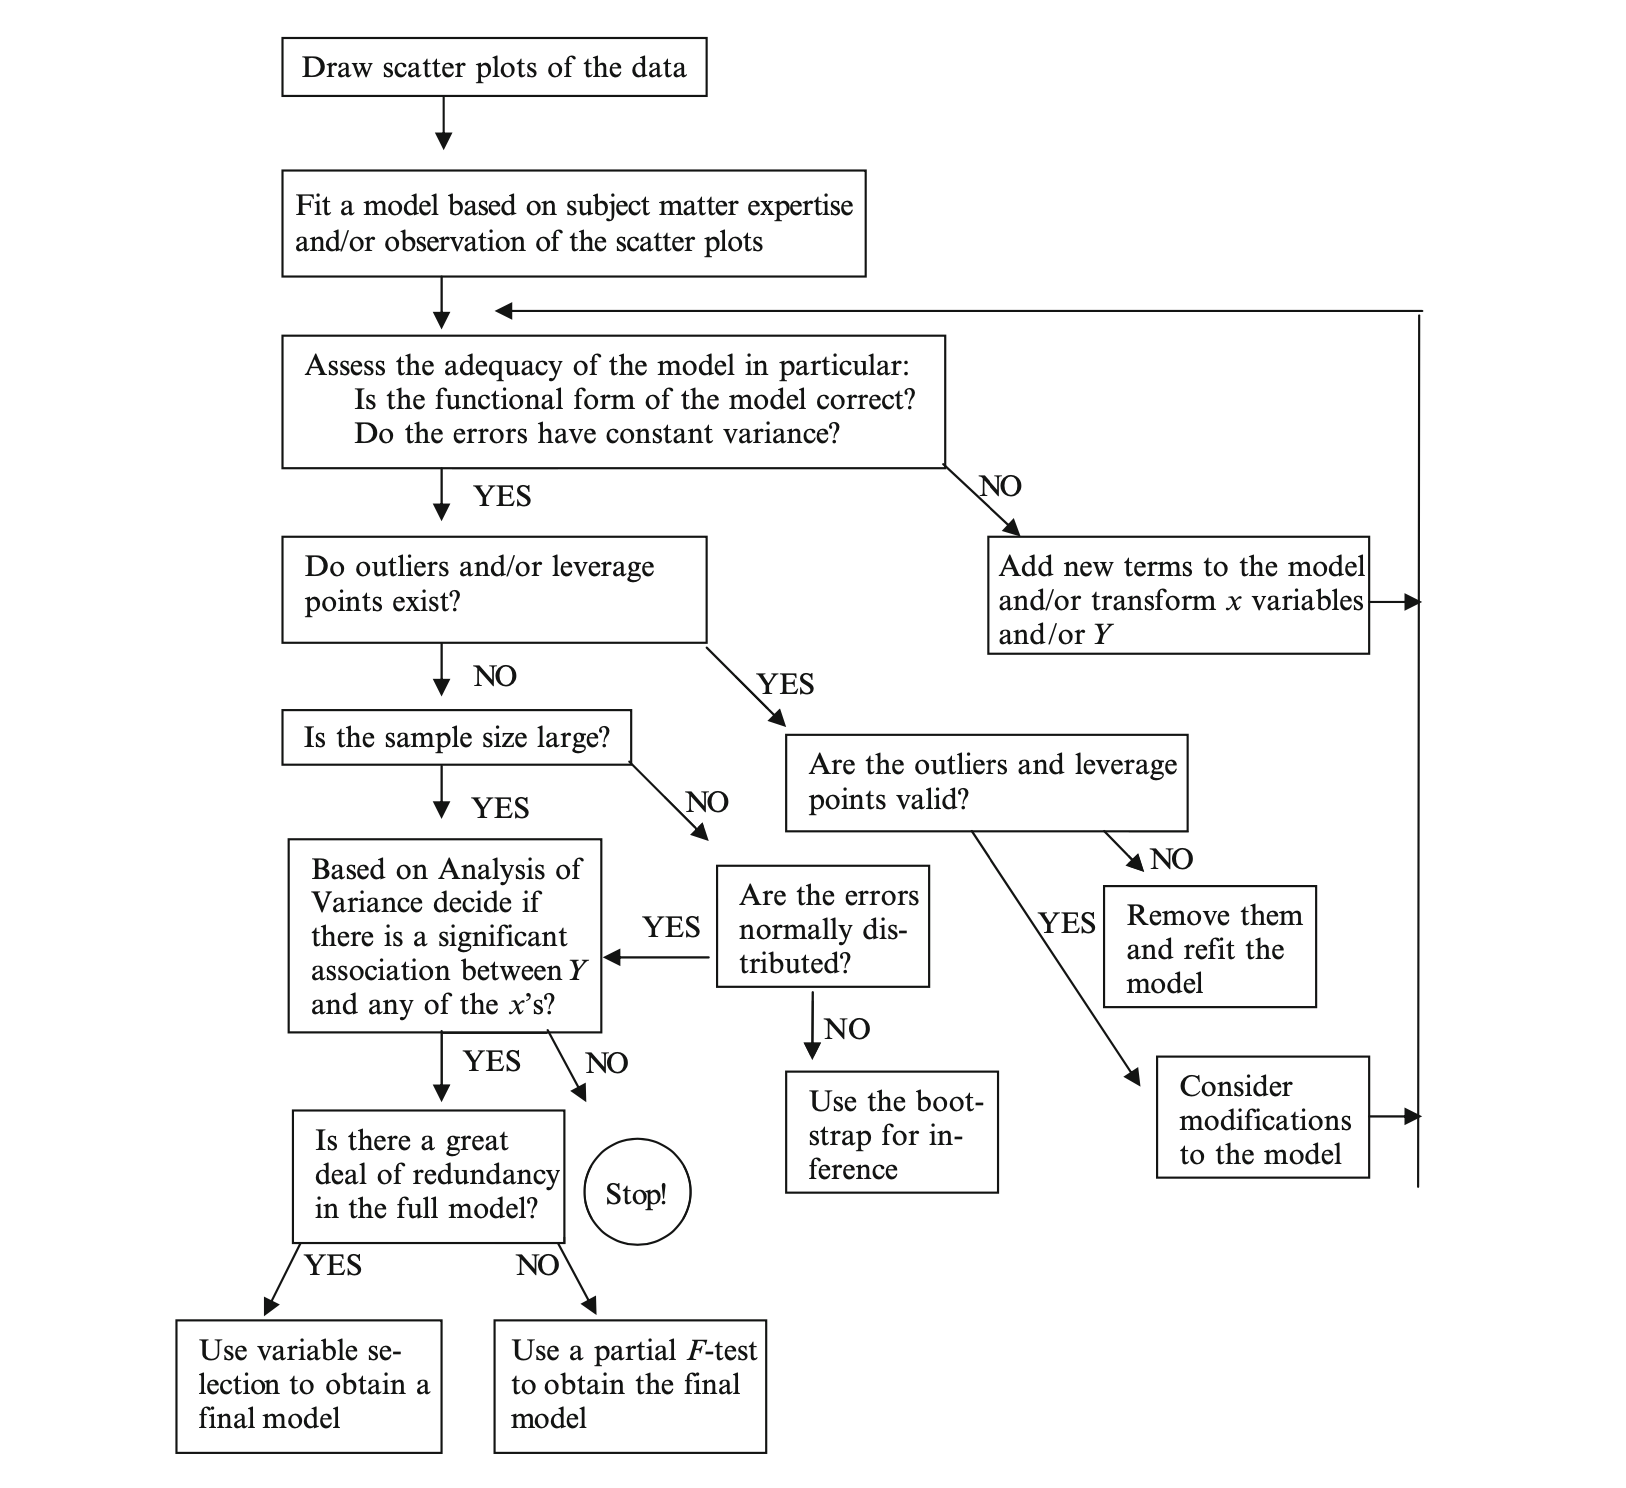
\includegraphics[width=\textwidth]{./images/data-analysis-flow}
%   \caption{Data Analysis Flow}
%   \label{data-analysis-flow}
% \end{figure}
\end{document}